\section{Introduction}

Hurwitz numbers are enumerations of branched morphisms between Riemann surfaces with fixed numerical data. They go back to work by Adolf Hurwitz in the 1890s~\cite{hurwitz1892algebraische} and are now important invariants in enumerative geometry. 
They admit various equivalent descriptions in the language of different areas of mathematics, e.g., as shown by Hurwitz in his above-mentioned work, they can be computed by an enumeration of transitive factorisations in the symmetric group. This equivalence gives rise to a deep connection between Hurwitz theory and the representation theory of the symmetric group; it will also play a key role in the present work. Moreover, Hurwitz numbers are closely related to the algebraic topology underlying Riemann surfaces, since they turn out to be \textit{topological invariants}. While the theory of Hurwitz numbers has been dormant for most of the 20th century, the close relationship between Hurwitz and Gromov--Witten theory discovered in the 1990s has rekindled interest in these enumerative invariants and led to several exciting developments.\vspace{\baselineskip}

\subsection{Hurwitz numbers, Gromov--Witten theory and variants}
When studying relations between Hurwitz numbers and Gromov--Witten theory, certain classes of Hurwitz numbers with particularly well--behaved structures take center stage. Among these classes are so-called \textit{double Hurwitz numbers}, which are defined as follows.

\begin{defi}[Double Hurwitz numbers]\label{def-hur}
Let $g\ge0$ be a non-negative integer, $n>0$ a positive integer and $\mu,\nu$ partitions of $n$. Moreover, we fix $p_1,\dots,p_b\in\mathbb{P}^1$, where $b=2g-2+\ell(\mu)+\ell(\nu)$. Then, we define a cover of type $(g,\mu,\nu)$ to be a map $f\colon S\to\mathbb{P}^1$, such that
\begin{itemize}
    \item $S$ is a connected Riemann surface of genus $g$;
    \item the ramification profile of $0$ is $\mu$;
    \item the ramification profile of $\infty$ is $\nu$;
    \item the ramification profile of $p_1,\dots,p_b$ is $(2,1\dots,1)$.
\end{itemize}
Two covers $f\colon S\to\mathbb{P}^1$ and $f'\colon S'\to\mathbb{P}^1$ are called equivalent if there exists a homeomorphism $g\colon S\to S'$, such that $f= f'\circ g$.

Then, we define \textbf{double Hurwitz numbers} as
\begin{equation*}
    h_g(\mu,\nu)=\sum_{[f]}\frac{1}{|\mathrm{Aut}(f)|},
\end{equation*}
where the sum runs over all equivalence classes of covers of type $(g,\mu,\nu)$.

When $\nu=(1,\dots,1)$, we call $h_g(\mu,\nu)$ a \textbf{single Hurwitz number} and denote it by~$h_g(\mu)$.
\end{defi}

At the core of the relationship between double Hurwitz numbers and Gromov--Witten theory is a polynomial structure in the prescribed ramification data of these enumerative invariants. First discovered in the seminal work of Goulden, Jackson and Vakil in~\cite{GJV05}, double Hurwitz numbers exhibit a \textit{piecewise polynomial} behaviour. More precisely, we consider the space \begin{equation*}
    \mathcal{H}_{m.n}\coloneqq\{(\mu,\nu)\in\mathbb{N}^m\times\mathbb{N}^n\mid \sum \mu_i=\sum \nu_j\}
\end{equation*}
of partitions $(\mu,\nu)$ of fixed lengths $m,n$ and of the same size. For fixed $g$, we consider the map
\begin{align*}
    h_g\colon \mathcal{H}_{m,n}&\to\mathbb{Q}\\
    (\mu,\nu)&\mapsto h_g(\mu,\nu)
\end{align*}
which parametrises double Hurwitz numbers.

The authors of~\cite{GJV05} showed that there exists a hyperplane arrangement $\mathcal{R}_{m,n}$ in $\mathcal{H}_{m,n}$ (called the resonance arrangement), such that the map $h_g$ restricted to each connected component (called \textit{chamber}) of $\mathcal{H}_{m,n}\backslash\mathcal{R}_{m,n}$ may be represented as a polynomial in the entries of $\mu$ and $\nu$. In~\cite{SSV08, CJM11, Joh15}, the natural question of how the polynomials differ from chamber to chamber was studied. It was observed that there is a recursive structure in the sense that this difference can be expressed by double Hurwitz numbers with smaller input data. This is called a \textit{wall-crossing formula}.

We want to highlight the work in~\cite{CJM11}, in which a graph theoretic approach towards the polynomiality of double Hurwitz numbers was established. The key technique in this paper revolves around the field of \textit{tropical geometry}. Tropical geometry is a relatively new field of mathematics, which may be described as a combinatorial shadow of algebraic geometry. The tropical geometry perspective allows to degenerate algebraic curves to certain metric graphs that are called \textit{tropical curves}. In this manner, branched morphisms between Riemann surfaces are \textit{tropicalised} to maps between tropical curves that are called \textit{tropical covers}. Motivated by this point of view, a combinatorial interpretation of double Hurwitz numbers in terms of tropical covers was derived in~\cite{CJM10}, which laid the groundwork for the analysis of the polynomial behaviour of double Hurwitz numbers undertaken in~\cite{CJM11}. In particular, by proceeding along an intricate combinatorial analysis of tropical covers in different chambers, the authors of~\cite{CJM11} were able to derive the desired wall-crossing structure.

In the past years, several variants of Hurwitz numbers have appeared in the literature in a plethora of different contexts. Among the most prominent ones are so-called \textit{pruned Hurwitz numbers}~\cite{do2018pruned,hahn2020bi}, \textit{monotone Hurwitz numbers}~\cite{goulden2014monotone}, \textit{strictly monotone Hurwitz numbers}~\cite{kazarian2015virasoro}, \textit{completed cycles Hurwitz numbers}~\cite{okounkov2006gromov} and many more. For all of these variants the piecewise polynomiality of the double Hurwitz numbers analogue was established and for the majority a wall-crossing structure as well (see e.g.~\cite{zbMATH06791415, hahn2018wall,hahn2020wall,shadrin2012double}).

While classical Hurwitz theory deals with the enumeration of branched morphisms between \textit{orientable surfaces}, it is very natural to ask for an analogous theory for non-orientable surfaces. Such a new and exciting theory for so-called \textit{$b$-Hurwitz numbers} was introduced in~\cite{chapuy2020non}.

\subsection{Twisted Hurwitz numbers}\label{sec-twistedsingle}
The construction of $b$-Hurwitz numbers is based on the following idea:  Let $\overline{\mathbb{H}}$ be the compactified complex upper half-plane of $\mathbb{P}^1$ and $\mathcal{J}$ the corresponding natural involution on $\mathbb{P}^1$. A generalised branched covering is a covering $f\colon S\to\overline{\mathbb{H}}$ where $S$ is a not-necessarily connected compact orientable surface with orientation double cover $\hat{S}$, such that $f$ may be ``lifted'' to a branched covering $\hat{S}\to\mathbb{P}^1$. We give a precise formulation in~\cref{sec:twistdoub}. Via these generalised coverings the authors of~\cite{chapuy2020non} introduce a new one-parameter deformation of classical Hurwitz numbers called $b$-Hurwitz numbers in reference to the $b$-conjecture by Goulden and Jackson in the context of Jack polynomials~\cite{goulden1996connection}. In order to obtain $b$-Hurwitz numbers, the authors of~\cite{chapuy2020non} associate a non-negative integer $\nu_p(f)$ to any generalised branched covering $f$ which ``measures'' the non-orientability of the the surface $\hat{S}$. This non-negative integer is zero if and only if $\hat{S}$ is orientable. Based on this idea $b$-Hurwitz numbers are defined -- depending on a \textit{measure of non-orientability} $p$ -- as a sum over generalised branched coverings weighted by $b^{\nu_p(f)}$. Thus, one obtains a Hurwitz-type enumeration for any value of $b$. For example, under the convention that $0^0=1$, one  recovers classical Hurwitz numbers for $b=0$. For $b=1$, one obtains enumerations of generalised branched coverings which are called \textit{twisted Hurwitz numbers}. This is the case we study in the present paper.

The term twisted Hurwitz numbers was coined in~\cite{BF21} in the context of \textit{surgery theory}. Surgery theory studies the construction of new manifolds from given ones via cutting and gluing, such that key properties are preserved. In~\cite{BF21}, the enumeration of decompositions of a given surface with boundary and marked points is studied. The term \textit{twisted} is motivated by the fact in~\cite{BF21} gluings are performed with respect to a twist of the natural boundary orientations. It was proved in~\cite{BF21} that the enumeration of certain decompositions with respect to such a twist may be computed in terms of factorisations in the symmetric group, reminiscent of Hurwitz' result in his original work~\cite{hurwitz1892algebraische}. More precisely, we fix the involution $$\tau= (1\;\; n+1) (2 \;\;n+2) \ldots (n \;\;2n)\in \mathbb{S}_{2n},$$ and use the notation
\begin{equation*}
    B_n=C(\tau)=\{\sigma \in \mathbb{S}_{2n} \mid  \sigma \tau \sigma^{-1}=\tau\}, \; C^\sim(\tau)=\{\sigma \in \mathbb{S}_{2n} \mid  \tau \sigma \tau^{-1} = \tau \sigma \tau =  \sigma^{-1}\},
\end{equation*}
where $B_n$ is the hyperoctahedral group. We further define the subset $B^\sim_n \subset C^\sim(\tau)$ consisting of those permutations that have no self-symmetric cycles (see \cite[Lemma~2.1]{BF21}). We then set, for a partition $\lambda$ of $n$,  $B^\sim_\lambda\subset B^\sim_n$ to consist of those permutations that have $2\ell(\lambda)$ cycles, two of length $\lambda_i$ for each i, that pair up under conjugation with~$\tau$. We are now ready to define \textbf{twisted single Hurwitz numbers} in terms of the symmetric group.

\begin{defi}[Twisted single Hurwitz numbers,~\cite{BF21}]
\label{def:twisthur}
Fix a partition $\lambda$ of $n$ and a number $b$ (the number of transpositions).
Then define
\begin{align*}
\tilde{h}_{b}(\lambda)= \frac{1}{n!}\sharp \Big\{(\sigma_1,\ldots,\sigma_b) \mid  \sigma_s=(i_s\;\;j_s),\, j_s\neq \tau(i_s),\, \sigma_1\ldots\sigma_b (\tau\sigma_b\tau)\ldots (\tau\sigma_1\tau) \in B^{\sim}_\lambda\Big\}.
\end{align*}
\end{defi}

Maybe surprisingly, it was then proved in \cite[Theorem 3.2]{BF21} that these numbers coincide with $b$-Hurwitz numbers for $b=1$ by showing that the generating series of both invariants satisfy the same PDE with equal initial data.

\subsection{Tropical geometry of twisted Hurwitz numbers} 
The present paper develops a tropical theory of twisted Hurwitz numbers and demonstrates some first applications. In~\cref{sec:twistdoub}, we define a generalisation of~\cref{def:twisthur} to twisted double Hurwitz numbers $\tilde{h}_g(\mu,\nu)$ which by the same arguments as in \cite[Theorem 3.2]{BF21} coincides with $b$-Hurwitz numbers for $b=1$. This generalisation arises naturally from the symmetric group expression for twisted single Hurwitz numbers. Moreover, we define in~\cref{sec:troptwist} a tropical analogue of twisted double Hurwitz numbers in terms of tropical covers. We prove in~\cref{sec:corr} that twisted double Hurwitz numbers coincide with their tropical counterpart, thus giving a tropical correspondence theorem for these enumerative invariants. This allows us to derive a purely graph-theoretic interpretation of twisted double Hurwitz numbers in~\cref{sec:monodr} by reinterpreting the tropical covers as directed graphs.
Finally, we employ this expression of twisted double Hurwitz numbers as a weighted enumeration of directed graphs to study the polynomiality of twisted Hurwitz numbers in~\cref{sec:poly}. Finally, we discuss the wall-crossing behaviour of twisted Hurwitz numbers.

\section{Twisted double Hurwitz numbers}
\label{sec:twistdoub}
In this section, we define twisted double Hurwitz numbers as a factorization problem in the symmetric group, generalizing the case of single twisted Hurwitz numbers discussed in \cref{sec-twistedsingle}. We use the notation of \cref{sec-twistedsingle}. To begin with, we recall that

\begin{equation*}
     C^\sim(\tau)=\{\sigma\in \mathbb{S}_{2n}  \mid  \tau \sigma \tau^{-1} = \tau \sigma \tau =  \sigma^{-1}\}.
\end{equation*}

It was proved in \cite[Lemma 2.1]{BF21} for $\sigma \in C^\sim(\tau)$ with the decomposition in cycles $\sigma=c_1\cdots c_m$, we have for any $i$ that either
\begin{itemize}
    \item there exists $j\neq i$ with $\tau c_i\tau=c_j^{-1}$ or
    \item we have $\tau c_i\tau=c_i^{-1}$ and $c_i$ has even length.
\end{itemize}
In the first case, $c_i$ and $c_j$ are called \textit{$\tau$-symmetric}, while in the second case $c_i$ is called \textit{self-symmetric}. As mentioned above, we denote by $B_n^\sim\subset C^\sim(\tau)$ the set of permutations without self-symmetric cycles and by $B^\sim_\lambda\subset B^\sim_n$ the set of permutations in $B^\sim_n$ with $2\ell(\lambda)$ cycles and for each $i$ two cycles of length $\lambda_i$ that are $\tau$-symmetric.

\begin{defi}[Cycle type]
Let $\sigma\in B^{\sim}_n$. We denote its cycle type by $C(\sigma)$, which is a partition of $2n$ recording the lengths of the cycles of $\sigma$.
\end{defi}

For a partition $\mu$ of $n$ we denote by $2\mu$ the partition of $2n$ with twice as many parts, where each part is repeated once.

We may now define twisted double Hurwitz numbers generalising~\cref{def:twisthur}.

\begin{defi}[Twisted double Hurwitz numbers]
\label{def:twisthurdou}
Let $g\ge0,n>0$ and $\mu,\nu$ partitions of $n$. We define $C_g(\mu,\nu)$ as the set of tuples $(\sigma_1,\eta_1,\dots,\eta_b,\sigma_2)$,
such that we have:
\begin{enumerate}
    \item $b=\frac{2g-2+2\ell(\mu)+2\ell(\nu)}{2}>0$,
    \item $C(\sigma_1)=2\mu$, $C(\sigma_2)=2\nu$, $\eta_i$ are transpositions satisfying $\eta_i\neq \tau \eta_i \tau$,
    \item $\sigma_1\in B^\sim_\mu$,
    \item $\eta_b\cdots\eta_1\sigma_1(\tau\eta_1\tau)\cdots(\tau\eta_b\tau)=\sigma_2$,
    \item the subgroup 
    $$\langle \sigma_1,\eta_1,\ldots,\eta_{b},\tau \eta_1\tau, \ldots,\tau\eta_b\tau,\sigma_2\rangle$$ acts transitively on the set $\{1,\ldots,2d\}$.
\end{enumerate}
Then, we define the associated \textit{twisted double Hurwitz number} as
\begin{equation*}
    \tilde{h}_{g}(\mu,\nu)=\frac{1}{(2n)!!}|C_g(\mu,\nu)|.
\end{equation*}
When we drop the transitivity condition, we obtain possibly disconnected twisted double Hurwitz numbers which we denote $\tilde{h}_{g}^\bullet(\mu,\nu)$.
\end{defi}

\begin{rema}[Conventional differences]
Compared with the definition of twisted single Hurwitz numbers in \cref{def:twisthur}, there are two conventional differences:
\begin{enumerate}
    \item Rather than the number of transpositions, we use the genus (of the source of a twisted tropical cover, see \cref{def-twistedtropcover}) as subscript in the notation. In the usual case of Hurwitz numbers (without twisting) counting covers, this corresponds to the genus of the source curves. By the Riemann-Hurwitz formula, the genus $g$ and the number $b$ of transpositions (i.e.\ simple branch points) are related via
    $$b=\frac{2g-2+2\ell(\mu)+2\ell(\nu)}{2}.$$

    \item We choose to normalize with the factor $\frac{1}{(2n)!!}$ rather than $\frac{1}{n!}$. This leads to nicer formulae and structural results.
\end{enumerate}

\end{rema}
\begin{rema}[Connectedness and transitivity]
    As noted above, one can also drop the transitivity condition (5) in \cref{def:twisthurdou} to obtain $\tilde{h}_g^\bullet(\mu,\nu)$. On the tropical side, this amounts to allowing disconnected tropical curves as source of a twisted tropical cover, see \cref{def-twistedtropcover}. In this setting, it can happen that a disconnected twisted tropical cover contains two twisted components which both just correspond to a single edge without any interior vertex. This also happens in the connected case if we allow $b=0$. For this case, one has to adapt the tropical multiplicity we set in \cref{def:twisttrophn}: a twisted tropical cover which consists of a pair of twisted single edges of weight $\mu$ each has multiplicity $\frac{1}{\mu}$. With this adaption, one can easily generalize our results to the disconnected case.
\end{rema}

As mentioned in the introduction, twisted Hurwitz numbers first appeared in the Hurwitz theory of non-orientable surfaces. More precisely, we denote by $\mathcal{J}\colon\mathbb{P}^1\to\mathbb{P}^1$ the complex conjugation, by $\mathbb{H}\coloneqq\{z\in\mathbb{C}\mid\mathrm{Im}(z)\ge0\}$ the complex upper half-plane and by $\overline{\mathbb{H}}\coloneqq\mathbb{H}\cup\{\infty\}$ the compactified complex upper half-plane. Moreover, we denote by $\pi\colon\mathbb{P}^1\to\overline{\mathbb{H}}$ the quotient map.

We call continuous maps $f\colon S\to\overline{\mathbb{H}}$ \textit{generalised branched coverings}, if $S$ is a not-necessarily orientable surface and there exists a further map $\hat{f}\colon \hat{S}\to\mathbb{P}^1$ with
    \begin{enumerate}
        \item $p\colon\hat{S}\to S$ is the orientation double cover,
        \item $\pi\circ\hat{f}=f\circ p$,
        \item all the branch points of $\hat{f}$ are real.
    \end{enumerate}
Let $\mathcal{T}\colon \hat{S}\to\hat{S}$ be an orientation reversing involution without fix points, such that $p\circ \mathcal{T}=p$. Then, the second condition of $\hat{f}$ may be reformulated as $\hat{f}\circ\mathcal{T}=\mathcal{J}\circ \hat{f}$. As $\mathcal{T}$ has no fixed points, for any branch points $c\in\mathbb{P}^1_{\mathbb{R}}\subset\mathbb{P}^1$ of $\hat{f}$, the points in its pre-image come in pairs $(a,\mathcal{T}(a))$ with the same ramification index. Thus, the degree of $\hat{f}$ is even and the ramification profile of $c$ repeats any entry twice, e.g. $(\lambda_1,\lambda_1,\dots,\lambda_s,\lambda_s)$. We then say that $f$ has ramification profile $(\lambda_1,\dots,\lambda_s)$ at $\pi(s)\in\partial\overline{\mathbb{H}}$. We further call two generalised branched coverings $f_1$ and $f_2$ equivalent if their lifts $\hat{f_1}$ and $\hat{f_2}$ are, and denote the equivalence class of $f$ by $[f]$. 

\begin{defi}\label{def-nonoriented}
    Let $g\ge0$, $n>0$, $\mu,\nu$ partitions of $n$. Let $b=\frac{2g-2+2\ell(\mu)+2\ell(\nu)}{2}$ and fix $p_1,\dots,p_b$ pairwise distinct real points on $\overline{\mathbb{H}}$. We define $G_g(\mu,\nu)$ as the set of equivalence classes $[f]$ of generalised branched coverings $f\colon S\to\overline{\mathbb{H}}$, such that
    \begin{itemize}
        \item $f$ is of degree $n$,
        \item $f$ has ramification profile $\mu$ over $0$ and $\nu$ over $\infty$,
        \item $f$ has ramification profile $(2,1,\dots,1)$ over $p_i$.
    \end{itemize}
    Then, we define $1$-Hurwitz numbers as
    \begin{equation*}
        h^1_g(\mu,\nu)=\sum_{[f]\in G_g(\mu,\nu)}\frac{1}{|\mathrm{Aut}(f)|}.
    \end{equation*}
\end{defi}
The parameter $g$ used here is not equal to the genus of the surface $S$, this is $g'=\frac{g+1}{2}.$

The following was proved in \cite[Theorem 3.2]{BF21} for $\nu=(1,\dots,1)$. However, the same approach works for arbitrary $\nu$. In particular, the idea is that in \cite[Theorem 6.5]{chapuy2020non} a recursion of $b$--Hurwitz numbers was derived. Moreover, twisted Hurwitz numbers were proved to satisfy a recursion in \cite[Theorem 2.12]{BF21}. It turns out that these recursions only differ by a factor of $2$. The same argument as in the proof of \cite[Theorem 3.2]{BF21} proves the following result.

\begin{theo}
    Let $g\ge0$, $n>0$ and $\mu$, $\nu$ partitions of $d$. Then, we have
    \begin{equation*}
        h^1_g(\mu,\nu)=2^{-b}\tilde{h}_g^{\bullet}(\mu,\nu).
    \end{equation*}
\end{theo}

\section{Tropical twisted covers and twisted Hurwitz numbers}
\label{sec:troptwist}

In~\cite{CJM10}, tropical Hurwitz numbers have been introduced as a count of tropical covers, parallel to the count of covers of algebraic curves from \cref{def-hur}. We start by recalling the basic notions of tropical curves and covers. Then we introduce twisted tropical covers, which can roughly be viewed as tropical covers with an involution. By fixing branch points, we produce a finite count of twisted tropical covers for which we show in the following section that it coincides with the corresponding twisted double Hurwitz number. Readers with a background in the theory of tropical curves are pointed to the fact that we only consider explicit tropical curves in the following, i.e.\ there is no genus hidden at vertices.

\begin{defi}[Abstract tropical curves]
An abstract tropical curve is a connected graph $\Gamma$ with the following data:
\begin{enumerate}
    \item The vertex set of $\Gamma$ is denoted by $V(\Gamma)$ and the edge set of $\Gamma$ is denoted by $E(\Gamma)$.
    \item The $1$-valent vertices of $\Gamma$ are called \textit{leaves} and the edges adjacent to leaves are called \textit{ends}.
    \item The set of edges $E(\Gamma)$ is partitioned into the set of ends $E^\infty(\Gamma)$ and the set of \textit{internal edges} $E^0(\Gamma)$.
    \item There is a length function
    \begin{equation*}
        \ell\colon E(\Gamma)\to\mathbb{R}\cup\{\infty\},
    \end{equation*}
    such that $\ell^{-1}(\infty)=E^\infty(\Gamma)$.
\end{enumerate}
The genus of an abstract tropical curve $\Gamma$ is defined as the first Betti number of the underlying graph, i.e.\ $g=1+\# E^0(\Gamma)-\# V(\Gamma)$. An isomorphism of abstract tropical curves is an isomorphism of the underlying graphs that respects the length function. The combinatorial type of an abstract tropical curve is the underlying graph without the length function.
\end{defi}

We are now ready to define the notion of a tropical cover. We restrict to the case where the target $\Gamma_2$ is a subdivided version of $\mathbb{R}$, i.e.\ a line with some $2$-valent vertices.

\begin{defi}[Tropical covers]
A tropical cover of a subdivided version of $\mathbb{R}$, $\Gamma_2$, is a surjective harmonic map between abstract tropical curves $\pi\colon \Gamma_1\to\Gamma_2$, i.e.:
\begin{enumerate}
    \item We have $\pi(V(\Gamma_1))\subset V(\Gamma_2)$.
    \item Let $e\in E(\Gamma_1)$. Then, we interpret $e$ and $\pi(e)$ as intervals $[0,\ell(e)]$ and $[0,\ell(\pi(e))]$ respectively. We require $\pi$ restricted to $e$ to be a bijective integer linear function $[0,\ell(e)]\to[0,\ell(\pi(e))]$ given by $t\mapsto \omega(e)\cdot t$, with $\omega(e) \in \mathbb{Z}$. If $\pi(e)\in V(\Gamma_2)$, we define $\omega(e)=0$. We call $\omega(e)$ the \textit{weight} of $e$.
    \item For a vertex $v\in V(\Gamma_1)$, we denote by $\mathrm{Inc}(v)$ the set of incoming edges at $v$ (edges adjacent to $v$ mapping to the left of $\pi(v)$) and by $\mathrm{Out}(v)$ the set of outgoing edges at $v$ (edges adjacent to $v$ mapping to the right of $\pi(v)$). We then require
    \begin{equation*}
            \sum_{e\in\mathrm{Inc}(v)}\omega(e)=\sum_{e\in\mathrm{Out}(v)}\omega(e).
    \end{equation*}
    This number is called the local degree of $\pi$ at $v$.
    We call this equality the \textit{harmonicity} or \textit{balancing condition}.
    For a point $v$ in the interior of an edge $e$ of $\Gamma_1$, the local degree of $\pi$ at $v$ is defined to be the weight $\omega(e)$.
\end{enumerate}
Moreover, we define the \textit{degree} of $\pi$ as the sum of local degrees of all preimages in $\Gamma_1$ of a given point of $\Gamma_2$. The degree is independent of the choice of point of $\Gamma_2$. This follows from the harmonicity condition.

For any end $e$ of $\Gamma_2$, we define a partition $\mu_e$ as the partition of weights of ends of~$\Gamma_1$ mapping to $e$. We call $\mu_e$ the \textit{ramification profile} of $e$.

We call two tropical covers $\pi_1\colon\Gamma_1\to\Gamma_2$ and $\pi_2\colon\Gamma_1'\to\Gamma_2$ equivalent if there exists an isomorphism $g\colon\Gamma_1\to\Gamma_1'$ of metric graphs, such that $\pi_2\circ g=\pi_1$.
\end{defi}

\begin{defi}[Twisted tropical covers]\label{def-twistedtropcover}
We define a twisted tropical cover of type $(g,\mu,\nu)$ to be a tropical cover $\pi\colon\Gamma_1\to\Gamma_2$ with an involution $\iota\colon\Gamma_1\to\Gamma_1$ which respects the cover $\pi$, such that:
\begin{itemize}
    \item The target $\Gamma_2$ is a subdivided version of $\mathbb{R}$ with vertices $\{p_1,\dots,p_b\}=V(\Gamma_2)$, where $p_i<p_{i+1}$. Here, $b=\frac{2g-2+2\ell(\mu)+2\ell(\nu)}{2}$. These points are called the \emph{branch points}.
    \item There are $\ell(\mu)$ pairs of ends mapping to $(-\infty,p_1]$ with weights $\mu_1,\dots,\mu_{\ell(\mu)}$ and $\ell(\nu)$ pairs of ends mapping to $[p_b,\infty)$ with weights $\nu_1,\ldots,\nu_{\ell(\nu)}$.
    \item in the preimage of each point $p_i$, there are either two $3$-valent vertices or one $4$-valent vertex.
    \item the edges adjacent to a $4$-valent vertex all have the same weight.
    \item the fixed locus of $\iota$ is exactly the set of $4$-valent vertices.
\end{itemize}
\end{defi}

\begin{defi}[Quotient graph $\Gamma/\iota$]
Let $\pi\colon \Gamma\to \mathbb{R}$ be a twisted tropical cover with involution $\iota\colon\Gamma\to\Gamma$. The involution $\iota$ induces a symmetric relation on the vertex and edge sets of $\Gamma$: We define for $v,v'\in V(\Gamma)$  (resp. $e,e'\in E(\Gamma)$) that $v\sim v'$ (resp. $e\sim_\iota e'$) if and only $\iota(v)=v'$ (resp. $\iota(e)=e'$). We define $\Gamma/\iota$ as the graph with vertex set $V(\Gamma)/\sim$ and edge set $E(\Gamma)/\sim$ with natural identifications. For $e=[e',e'']\in E(\Gamma/\iota)$ we define the length $\ell(e)$ as $\ell(e')=\ell(e'')$ and its weight $\omega(e)$ with respect to $\pi$ to be the weight $\omega(e')=\omega(e'')$.
\end{defi}

\begin{exam}
The graph on the left in~\cref{fig:extwist} shows a twisted tropical cover $\pi$ of type $(0,(4),(2,2))$. We fix $p_1=-5$ and $p_2=5$. The graph on the top represents the source curve $\Gamma_1$, whereas the graph $\Gamma_2$ on the bottom is $\mathbb{R}$ with two marked points $p_1$ and~$p_2$. The graph above is mapped to the graph below via the projection indicated by the arrow, e.g. the two left most edges of $\Gamma_1$ are each mapped to $(-\infty,-5)$. The green labels indicate the lengths of the corresponding edge. We have six unbounded edges of $\Gamma_1$, whose lengths we denote by $\infty$ and two bounded edges, each of length five and each mapped to $(-5,5)$. The graph $\Gamma_2$ has two unbounded edges corresponding to the intervals $(-\infty,-5)$ and $(5,\infty)$ and one bounded edge which corresponds to~$(-5,5)$. The red labels indicate the weights $\omega(e)$ of the corresponding edges $e$. For the two bounded edges of $\Gamma_1$, we see immediately that the corresponding weight has to be $2$, since $\ell(\pi(e))=\omega(e)\cdot \ell(e)$. For the unbounded edges the weight cannot be read off the difference of lengths of the original edge and its image. However, the choices of weights in~\cref{fig:extwist} satisfy the balancing condition. The involution $\iota$ can be visualized in the picture as the reflection along a horizontal line passing through the $4$-valent vertex. We can see that the picture
yields a twisted tropical cover of type $(0,(4),(2,2))$. On the right of~\cref{fig:extwist} the quotient graph $\Gamma/\iota$ is illustrated.
\end{exam}

\begin{defi}[Automorphisms]
    Let $\pi:\Gamma\rightarrow \mathbb{R}$ be a twisted tropical cover with involution $\iota:\Gamma\rightarrow \Gamma$. An automorphism of $\pi$ is a morphism of abstract tropical curves (i.e.\ a map of metric graphs) $f:\Gamma\rightarrow\Gamma$ respecting the cover and the involution, i.e.\ $\pi\circ f = \pi$ and $f\circ \iota = \iota \circ f$. We denote the group of automorphisms of $\pi$ by $\Aut(\pi)$.
\end{defi}

\begin{figure}
\tikzset{every picture/.style={line width=0.75pt}}     

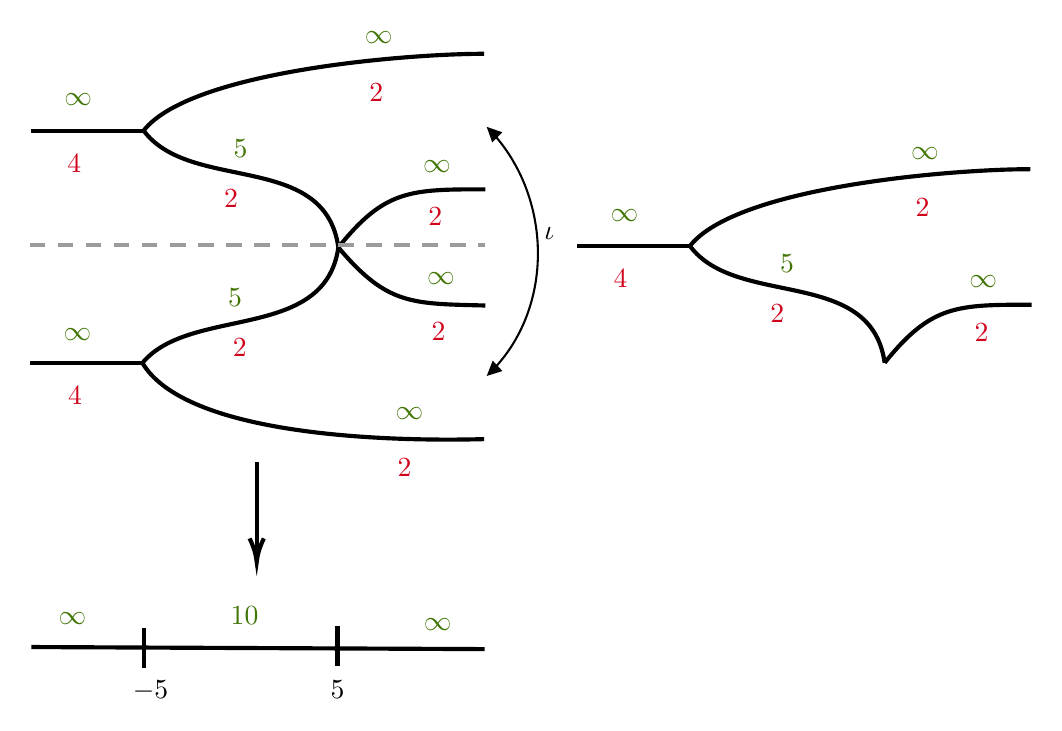
\begin{tikzpicture}[x=0.75pt,y=0.75pt,yscale=-1,xscale=1,scale=0.8]

\draw [line width=1.5]    (13.74,63.25) -- (81.59,63.25) ;
\draw [line width=1.5]    (81.59,63.25) .. controls (109.62,27.48) and (239.42,16.99) .. (286.62,16.99) ;
\draw [line width=1.5]    (81.59,63.25) .. controls (109.62,100.95) and (190.75,75.3) .. (198.86,133.6) ;
\draw [line width=1.5]    (13,203.18) -- (80.85,203.18) ;
\draw [line width=1.5]    (80.85,203.18) .. controls (108.88,250.22) and (245.32,250.22) .. (286.62,249.05) ;
\draw [line width=1.5]    (80.85,203.18) .. controls (109.62,168.59) and (190.75,190.74) .. (198.86,133.6) ;
\draw [line width=1.5]    (198.86,133.6) .. controls (226.88,98.62) and (242.37,98.62) .. (287.36,98.62) ;
\draw [line width=1.5]    (198.86,133.6) .. controls (228.36,168.59) and (243.11,167.42) .. (287.36,168.59) ;
\draw [line width=1.5]    (149.69,263.09) -- (149.69,320.05) ;
\draw [shift={(149.69,323.05)}, rotate = 270] [color={rgb, 255:red, 0; green, 0; blue, 0 }  ][line width=1.5]    (14.21,-4.28) .. controls (9.04,-1.82) and (4.3,-0.39) .. (0,0) .. controls (4.3,0.39) and (9.04,1.82) .. (14.21,4.28)   ;
\draw [line width=1.5]    (13.97,374.27) -- (286.88,375.52) ;
\draw [line width=1.5]    (81.59,386.77) -- (81.59,363.03) ;
\draw [line width=1.5]    (198.34,385.52) -- (198.34,361.78) ;
\draw [color={rgb, 255:red, 155; green, 155; blue, 155 }  ,draw opacity=1 ][line width=1.5]  [dash pattern={on 5.63pt off 4.5pt}]  (13,132) -- (287.36,132) ;
\draw    (290.57,63.44) .. controls (327.96,103.22) and (329.28,170.72) .. (290.02,209.26) ;
\draw [shift={(288.2,211)}, rotate = 317.09] [fill={rgb, 255:red, 0; green, 0; blue, 0 }  ][line width=0.08]  [draw opacity=0] (8.93,-4.29) -- (0,0) -- (8.93,4.29) -- cycle    ;
\draw [shift={(288.2,61)}, rotate = 44.8] [fill={rgb, 255:red, 0; green, 0; blue, 0 }  ][line width=0.08]  [draw opacity=0] (8.93,-4.29) -- (0,0) -- (8.93,4.29) -- cycle    ;
\draw [line width=1.5]    (342.74,132.74) -- (410.59,132.74) ;
\draw [line width=1.5]    (410.59,132.74) .. controls (438.62,96.98) and (568.42,86.48) .. (615.62,86.48) ;
\draw [line width=1.5]    (410.59,132.74) .. controls (438.62,170.44) and (519.75,144.79) .. (527.86,203.1) ;
\draw [line width=1.5]    (527.86,203.1) .. controls (555.88,168.11) and (571.37,168.11) .. (616.36,168.11) ;

\draw (73.28,392.91) node [anchor=north west][inner sep=0.75pt]    {$-5$};
\draw (192.34,392.91) node [anchor=north west][inner sep=0.75pt]    {$5$};
\draw (31.98,39.37) node [anchor=north west][inner sep=0.75pt]  [color={rgb, 255:red, 65; green, 117; blue, 5 }  ,opacity=1 ]  {$\infty $};
\draw (31.5,180.54) node [anchor=north west][inner sep=0.75pt]  [color={rgb, 255:red, 65; green, 117; blue, 5 }  ,opacity=1 ]  {$\infty $};
\draw (28.58,351.68) node [anchor=north west][inner sep=0.75pt]  [color={rgb, 255:red, 65; green, 117; blue, 5 }  ,opacity=1 ]  {$\infty $};
\draw (248.46,355.43) node [anchor=north west][inner sep=0.75pt]  [color={rgb, 255:red, 65; green, 117; blue, 5 }  ,opacity=1 ]  {$\infty $};
\draw (231.43,228.01) node [anchor=north west][inner sep=0.75pt]  [color={rgb, 255:red, 65; green, 117; blue, 5 }  ,opacity=1 ]  {$\infty $};
\draw (250.4,146.81) node [anchor=north west][inner sep=0.75pt]  [color={rgb, 255:red, 65; green, 117; blue, 5 }  ,opacity=1 ]  {$\infty $};
\draw (247.97,79.35) node [anchor=north west][inner sep=0.75pt]  [color={rgb, 255:red, 65; green, 117; blue, 5 }  ,opacity=1 ]  {$\infty $};
\draw (212.95,1.89) node [anchor=north west][inner sep=0.75pt]  [color={rgb, 255:red, 65; green, 117; blue, 5 }  ,opacity=1 ]  {$\infty $};
\draw (133.97,66.85) node [anchor=north west][inner sep=0.75pt]  [color={rgb, 255:red, 65; green, 117; blue, 5 }  ,opacity=1 ]  {$5$};
\draw (130.56,156.8) node [anchor=north west][inner sep=0.75pt]  [color={rgb, 255:red, 65; green, 117; blue, 5 }  ,opacity=1 ]  {$5$};
\draw (132.17,347.93) node [anchor=north west][inner sep=0.75pt]    {$\textcolor[rgb]{0.25,0.46,0.02}{10}$};
\draw (33.76,75.6) node [anchor=north west][inner sep=0.75pt]    {$\textcolor[rgb]{0.82,0.01,0.11}{4}$};
\draw (34.24,215.51) node [anchor=north west][inner sep=0.75pt]    {$\textcolor[rgb]{0.82,0.01,0.11}{4}$};
\draw (128.13,96.84) node [anchor=north west][inner sep=0.75pt]    {$\textcolor[rgb]{0.82,0.01,0.11}{2}$};
\draw (133.48,186.78) node [anchor=north west][inner sep=0.75pt]    {$\textcolor[rgb]{0.82,0.01,0.11}{2}$};
\draw (232.72,259.24) node [anchor=north west][inner sep=0.75pt]    {$\textcolor[rgb]{0.82,0.01,0.11}{2}$};
\draw (253.15,176.79) node [anchor=north west][inner sep=0.75pt]    {$\textcolor[rgb]{0.82,0.01,0.11}{2}$};
\draw (251.2,108.08) node [anchor=north west][inner sep=0.75pt]    {$\textcolor[rgb]{0.82,0.01,0.11}{2}$};
\draw (215.69,33.12) node [anchor=north west][inner sep=0.75pt]    {$\textcolor[rgb]{0.82,0.01,0.11}{2}$};
\draw (321.04,120) node [anchor=north west][inner sep=0.75pt]   [align=left] {$\displaystyle \iota $};
\draw (360.98,108.86) node [anchor=north west][inner sep=0.75pt]  [color={rgb, 255:red, 65; green, 117; blue, 5 }  ,opacity=1 ]  {$\infty $};
\draw (576.97,148.84) node [anchor=north west][inner sep=0.75pt]  [color={rgb, 255:red, 65; green, 117; blue, 5 }  ,opacity=1 ]  {$\infty $};
\draw (541.95,71.38) node [anchor=north west][inner sep=0.75pt]  [color={rgb, 255:red, 65; green, 117; blue, 5 }  ,opacity=1 ]  {$\infty $};
\draw (462.97,136.35) node [anchor=north west][inner sep=0.75pt]  [color={rgb, 255:red, 65; green, 117; blue, 5 }  ,opacity=1 ]  {$5$};
\draw (362.76,145.09) node [anchor=north west][inner sep=0.75pt]    {$\textcolor[rgb]{0.82,0.01,0.11}{4}$};
\draw (457.13,166.33) node [anchor=north west][inner sep=0.75pt]    {$\textcolor[rgb]{0.82,0.01,0.11}{2}$};
\draw (580.2,177.57) node [anchor=north west][inner sep=0.75pt]    {$\textcolor[rgb]{0.82,0.01,0.11}{2}$};
\draw (544.69,102.62) node [anchor=north west][inner sep=0.75pt]    {$\textcolor[rgb]{0.82,0.01,0.11}{2}$};
\end{tikzpicture}
\caption{A twisted tropical cover and its quotient graph.}
\label{fig:extwist}
\end{figure}

\begin{defi}[Twisted tropical Hurwitz number]
\label{def:twisttrophn}
We define the tropical twisted double Hurwitz 
number $\tilde{h}^{\trop}_g(\mu,\nu)$ to be  the weighted enumeration of equivalence classes of twisted tropical covers of type $(g,\mu,\nu)$, such that each equivalence class $[\pi\colon \Gamma\to\mathbb{R}]$ is counted with multiplicity
\begin{equation*}
    2^{b}\cdot \frac{1}{|\Aut(\pi)|}\cdot\prod_V (\omega_V-1)\prod_e\omega(e),
\end{equation*}
where $b$ is the number of branch points. Moreover, the first product goes over all $4$-valent vertices and $\omega_V$ denotes the weight of the adjacent edges, while the second product is taken over all internal edges of the quotient graph $\Gamma/\iota$ and $\omega(e)$ denotes their weights.
\end{defi}

\section{The Correspondence Theorem}
\label{sec:corr}
In this section, we show that  twisted double Hurwitz numbers coincide with their tropical counterparts.
In~\cref{con-twist}, we associate a twisted tropical cover to a tuple in the symmetric group counting towards a twisted Hurwitz number. In \cref{lem-outcomeconstruction}, we show that the outcome is indeed a twisted tropical cover. In \cref{thm-covermult}, we show that the multiplicity with which a twisted tropical cover is counted exactly equals the number of tuples that are mapped to it via~\cref{con-twist}. This proof builds on \cite[Theorem 2.12]{BF21}, where the cut-and-join operator for twisted Hurwitz numbers was derived.
The result is summed up in \cref{thm-corres}.

\begin{construction}
\label{con-twist}
Let $(\sigma_1,
\eta_1,\dots,\eta_b,\sigma_2)\in C_g(\mu,\nu)$. We let $\Gamma_2$ be $\mathbb{R}$ subdivided by $b$ vertices $p_i$ and construct a twisted tropical cover $\pi\colon\Gamma_1\to\Gamma_2$ associated to this tuple.

\begin{enumerate}
    \item First, we fix $p_1,\dots,p_b\in V(\Gamma_2)$ with $p_i<p_{i+1}$ and set $p_0=-\infty$ and $p_{b+1}=
    \infty$.
    \item We begin with $2\ell(\mu)$ ends over the interval $(-\infty,p_1]$, labelled by $\sigma_1^1,\dots,\sigma_1^{2\ell(\mu)}$, where $\sigma_1=\sigma_1^1\circ \ldots \circ \sigma_1^{2\ell(\mu)}$ is a decomposition of $\sigma_1$ into cycles. The action of $\tau$ on $\sigma_1$ yields an involution on these ends.
    \item By \cite[Theorem 2.14]{BF21}, the product
    \begin{equation}
    \label{equ:firststep}
        \eta_1\circ\sigma_1\circ(\tau\eta_1\tau) \tag{*}
    \end{equation}
    gives rise to three cases.
    \begin{enumerate}
        \item In this first case, we have four cycles $\sigma_1^1,\sigma_1^2,\sigma_1^3,\sigma_1^4$ of $\sigma_1$, such that
        \begin{equation*}
            \sigma_1^1\sigma_1^2\sigma_1^3\sigma_1^4\in B^{\sim}_n.
        \end{equation*}
        Then, the product in~\eqref{equ:firststep} joins two pairs of these cycles to two new cycles, e.g. $\sigma_1^1$, $\sigma_1^2$ to a new cycle $\eta_1\sigma_1^1\sigma_1^2\tau\eta_1\tau$; and $\sigma_1^3$, $\sigma_1^4$ to a new cycle $\eta_1\sigma_1^3\sigma_1^4\tau\eta_1\tau$.
        In this case, we create two vertices over $p_1$ each adjacent to two ends. We attach the ends that are joint via~\eqref{equ:firststep} to the same vertex. Moreover, we attach to each vertex two edges projecting to $[p_1,p_2]$ that are temporarily labeled by the corresponding cycles obtained from the join. Later, we replace this label by the length of the cycle as weight. This is illustrated in the following picture for the case that $\sigma_1^1$ is joined with $\sigma_1^2$ and $\sigma_1^3$ is joined with $\sigma_1^4$. Again, the action of $\tau$ on the permutation obtained from the join yields an involution of the tropical cover. 
        
        \begin{figure}[H]
        \scalebox{0.6}{
        \tikzset{every picture/.style={line width=0.75pt}}   
        \begin{tikzpicture}[x=0.75pt,y=0.75pt,yscale=-1,xscale=1]
        \draw    (51,30.5) -- (410.89,96.05) ;
        \draw    (51,156.22) -- (410.89,96.05) ;
        \draw    (410.89,96.05) -- (682,94.97) ;
        \draw    (51,178.78) -- (410.89,244.33) ;
        \draw    (51,304.5) -- (410.89,244.33) ;
        \draw    (410.89,244.33) -- (682,243.25) ;
        \draw    (50,370.5) -- (680,369.5) ;
        \draw    (411,360.5) -- (411,380.5) ;
        
        \draw (237.04,35.08) node [anchor=north west][inner sep=0.75pt]   [align=left] {$\displaystyle \sigma _{1}^{1}$};
        \draw (241.03,131.17) node [anchor=north west][inner sep=0.75pt]   [align=left] {$\displaystyle \sigma _{1}^{2}$};
        \draw (240.04,183.36) node [anchor=north west][inner sep=0.75pt]   [align=left] {$\displaystyle \sigma _{1}^{3}$};
        \draw (245.03,278.46) node [anchor=north west][inner sep=0.75pt]   [align=left] {$\displaystyle \sigma _{1}^{4}$};
        \draw (405,384) node [anchor=north west][inner sep=0.75pt]   [align=left] {$\displaystyle p_{1}$};
        \draw (505,68) node [anchor=north west][inner sep=0.75pt]   [align=left] {$\displaystyle \eta_1\sigma_1^1\sigma_1^2\tau\eta_1\tau$};
        \draw (510,215) node [anchor=north west][inner sep=0.75pt]   [align=left] {$\displaystyle \eta_1\sigma_1^3\sigma_1^4\tau\eta_1\tau$};
        \end{tikzpicture}}
        \end{figure}
           
        \item In the second case, we have two cycles $\sigma_1^1,\sigma_1^2$ of $\sigma_1$, such that
        \begin{equation*}
            \sigma_1^1\sigma_1^2\in B^{\sim}_n.
        \end{equation*}
        Then the product in~\eqref{equ:firststep} splits two cycles $\sigma_1^1$ and $\sigma_1^2$ each into two cycles, that we denote by $\sigma_1^{1,a},\sigma_1^{1,b}$ and $\sigma_1^{2,a},\sigma_1^{2,b}$ respectively. In this case, we create two vertices over $p_1$ each adjacent to one end labeled by $\sigma_1^1$ and $\sigma_1^2$ respectively. Moreover, we attach to each vertex two edges projecting to~$[p_1,p_2]$ that are temporarily labeled by the corresponding cycles obtained from the split, i.e.\ the new edges attached to the vertex adjacent to $\sigma_1^i$ are labeled by $\sigma_1^{i,a}$ and $\sigma_1^{i,b}$. We illustrate this construction in the following picture.
        
         \begin{figure}[H]
        \scalebox{0.6}{
        \tikzset{every picture/.style={line width=0.75pt}}
        \begin{tikzpicture}[x=0.75pt,y=0.75pt,yscale=-1,xscale=1]
        \draw    (682,29.5) -- (411,95.5) ;
        \draw    (682,156.22) -- (411,95.5) ;
        \draw    (411,95.5) -- (51,94.97) ;
        \draw    (682,178.78) -- (410,243.5) ;
        \draw    (683,303.5) -- (410,243.5) ;
        \draw    (410,243.5) -- (51,243.25) ;
        \draw    (50,370.5) -- (680,369.5) ;
        \draw    (411,360.5) -- (411,380.5) ;
        
        \draw (405,384) node [anchor=north west][inner sep=0.75pt]   [align=left] {$\displaystyle p_{1}$};
        \draw (215,66) node [anchor=north west][inner sep=0.75pt]   [align=left] {$\displaystyle \sigma _{1}^{1}$};
        \draw (216,253) node [anchor=north west][inner sep=0.75pt]   [align=left] {$\displaystyle \sigma _{1}^{2}$};
        \draw (528,31) node [anchor=north west][inner sep=0.75pt]   [align=left] {$\displaystyle \sigma _{1}^{1,a}$};
        \draw (529,131) node [anchor=north west][inner sep=0.75pt]   [align=left] {$\displaystyle \sigma _{1}^{1,b}$};
        \draw (529,186) node [anchor=north west][inner sep=0.75pt]   [align=left] {$\displaystyle \sigma _{1}^{2,a}$};
        \draw (530,282) node [anchor=north west][inner sep=0.75pt]   [align=left] {$\displaystyle \sigma _{1}^{2,b}$};
        \end{tikzpicture}
        }
        \end{figure}
        
        \item In the third case, we have two cycles $\sigma_1^1$ and $\sigma_1^2$ of $\sigma_1$ of the same length. Here, the product in~\eqref{equ:firststep} rearranges $\sigma_1^1$ and $\sigma_1^2$ into two new cycles $\tilde{\sigma}_1^1,\tilde{\sigma}_1^2$ of the same length. In this case, we create one vertex over $p_1$ that joins the two ends labeled by $\sigma_1^1,\sigma_1^2$. Moreover, we attach two new edges to this vertex that map to $[p_1,p_2]$ and that are labeled by $\tilde{\sigma}_1^1,\tilde{\sigma}_1^2$. 
        We illustrate this construction in the following picture.
    
        \begin{figure}[H]
        \tikzset{every picture/.style={line width=0.75pt}}
        \scalebox{0.6}{\begin{tikzpicture}[x=0.75pt,y=0.75pt,yscale=-1,xscale=1]
        \draw    (50,370.5) -- (659,369.5) ;
        \draw    (411,360.5) -- (411,380.5) ;
        \draw    (50,31) -- (411,161) ;
        \draw    (50,291) -- (411,161) ;
        \draw    (660,30) -- (411,161) ;
        \draw    (661,291) -- (411,161) ;
        
        \draw (405,384) node [anchor=north west][inner sep=0.75pt]   [align=left] {$\displaystyle p_{1}$};
        \draw (178,52) node [anchor=north west][inner sep=0.75pt]   [align=left] {$\displaystyle \sigma _{1}^{1}$};
        \draw (553,253) node [anchor=north west][inner sep=0.75pt]   [align=left] {$\displaystyle \widetilde{\sigma _{1}^{2}}$};
        \draw (555,40) node [anchor=north west][inner sep=0.75pt]   [align=left] {$\displaystyle \widetilde{\sigma _{1}^{1}}$};
        \draw (181,243) node [anchor=north west][inner sep=0.75pt]   [align=left] {$\displaystyle \sigma _{1}^{2}$};
        \end{tikzpicture}}
        \end{figure}

    \end{enumerate}
    In each case, we further extend all ends not attached to a vertex over $p_1$ to~$[p_1,p_2]$.
    \item We now take the permutation $\eta_1\sigma_1\tau\eta_1\tau$ and consider the product
    \begin{equation*}
        \eta_2(\eta_1\sigma_1\tau\eta_1\tau)\tau\eta_2\tau.
    \end{equation*}
    We proceed as in step (2) and create the corresponding vertices over $p_2$. Moreover, we proceed inductively for $\eta_i\eta_{i-1}\dots\eta_1\sigma_1\tau\eta_1\cdots\eta_i\tau$ until $i=b$. For $i=b$, we obtain ends that are labeled by the cycles of $\sigma_2$ and that project to $[p_b,\infty)$. This gives a map between graphs $\tilde{\pi}\colon\tilde{\Gamma_1}\to\Gamma_2$.
    \item The conjugation by $\tau$ induces a natural involution $
    \tilde{\iota}\colon\tilde{\Gamma}_1\to\tilde{\Gamma}_1$ that respects the map $\tilde{\pi}$.
    \item Next, for each edge $e$ of $\tilde{\Gamma}_1$, we replace the cycle labeling it by the length of this cycle. We consider this cycle length as the weight of $e$. 
\end{enumerate}
\end{construction}

\begin{lemma}\label{lem-outcomeconstruction}
Let $(\sigma_1,
\eta_1,\dots,\eta_b,\sigma_2)\in C_g(\mu,\nu)$. Perform~\cref{con-twist} to obtain $\pi\colon\Gamma_1\to\Gamma_2$. Then $\pi\colon\Gamma_1\to\Gamma_2$ is indeed a twisted tropical cover.
    \end{lemma}

\begin{proof}
    This follows from the fact that the lengths of cycles (which become weights of the cover) in the cut-and-join analysis add up as expected in the harmonicity condition. The involution is obtained from the action of $\tau$. The connectedness of $\Gamma_1$ follows from the transitivity condition in \cref{def:twisthurdou} (5).
\end{proof}

\begin{rema}
    Given a twisted tropical cover, we can label the edges recursively by cycles of a permutation $\sigma_1$ resp.\ of permutations of the form $\eta_1\sigma_1\tau\eta_1\tau$ and so on. In the following, we study how many ways there are to label the edges of a cover. This builds on \cite[Theorem 2.12]{BF21} which studies the cut-and-join analysis for the action of two partner transpositions. With this, we can determine the number of labels for the edges on the right of a vertex, if the edges on the left are already labeled. We obtain a recursive way to count the number of tuples that yield a given twisted tropical cover. This is detailed in \cref{thm-covermult}. Before, we count the number of ways to label the left ends of a twisted tropical cover.
\end{rema}

The following is a well-known fact (see e.g.~\cite{goulden1996connection}, Proposition 5.2). For the sake of completeness, we nevertheless include the short proof below.
\begin{lemma}
\label{lem-conjclass}
Let $\mu$ be a partition of $n$.
The cardinality of $B^\sim_\mu$ equals
$$ \frac{1}{2^{\ell(\mu)}} \frac{1}{\prod \mu_i} \frac{1}{|\Aut(\mu)|}(2n)!! .$$
\end{lemma}

\begin{proof}
We consider an ``empty'' permutation consisting of $2$ cycles of length $\mu_i$ for every $i$ such that each cycle contains $\mu_i$ placeholders. Then we count the possibilities to fill up the placeholders one by one with numbers from $1,\ldots,2n$.

For the first place, we have $2n$ options. 
Having chosen one placeholder to be $j$, the element $\tau(j)$ is not allowed to be in the same cycle. For that reason, if our cycle is not yet completed, we have $2n-2$ options to choose for the next place. If the cycle is completed, the involution $\tau$ requires us to fill up the partner cycle of length $1$ as $(\tau(j))$. Thus, we cannot choose $\tau(j)$ either as we fill up the first placeholder of the next cycle. We thus have $2n-2$ options again.

Recursively, we can see that we have $2n!!$ ways to fill our placeholders with numbers. This is not the right count yet, we have overcounted in multiple ways:
\begin{itemize}
    \item For every cycle and its partner cycle, it does not matter in which way we arranged the cycles, so we have to divide by a factor of $2$ of each entry of $\mu$, i.e.\ by $\frac{1}{2^{\ell(\mu)}}$.
    \item If $\mu$ has automorphisms, using the same argument, it does not matter how we arranged, so we have to divide by $\Aut(\mu)$.
    \item Finally, we overcounted for each cycle a factor of $\mu_i$, as we can cyclically exchange the entries in a cycle without changing the cycle.
\end{itemize}
Altogether, we obtain the claimed expression.
\end{proof}

\begin{exam}
Let $n=3$ and $\mu=(2,1)$. Then $\tau=(14)(25)(36)$.
The expression above yields $\frac{1}{2^2}\frac{1}{2\cdot 1}6!! = 6$.
The six elements in $B^{\sim}_\mu$ are
\begin{gather*}
    (12)(3)(45)(6), (13)(2)(46)(5), (15)(3)(24)(6), \\
    (16)(2)(34)(5), (23)(1)(56)(4), (26)(1)(53)(4).
\end{gather*}
\noindent
Let $n=3$ and $\mu=(3)$. The expression yields $\frac{1}{2}\frac{1}{3}6!!= 8$.
The eight elements in $B^{\sim}_\mu$ are
\begin{gather*}
    (123)(654), (132)(564), (126)(354), (162)(534), \\ 
    (135)(264), (153)(624), (156)(324), (165)(234).
\end{gather*}
\noindent
Let $n=2$ and $\mu=2$. The $\tau=(13)(24)$. The $\frac{1}{2}\frac{1}{2}4!!=2$ elements in $B^{\sim}_\mu$ are
$$ (12)(34), (14)(23).$$
\end{exam}

We are now ready to enumerate twisted factorisations that give rise to the same twisted tropical cover.

\begin{prop}\label{thm-covermult}
Given a twisted tropical cover $\pi\colon\Gamma\to\mathbb{R}$ with involution $\iota$ of type $(g,\mu,\nu)$. Then, the numbers of twisted factorisations in $C_g(\mu,\nu)$ giving rise to $(\pi,\iota)$ via~\cref{con-twist} is
\begin{equation*}
(2n)!!\cdot 2^{b}\cdot \prod_V (\omega_V-1)\prod_e\omega(e)\cdot \frac{1}{|\Aut(\pi)|},
\end{equation*}
where $b$ is the number of branch points. Here, the first product goes over all $4$-valent vertices of $\Gamma$ and $\omega_V$ denotes the weight of the adjacent edges, while the second product is taken over all internal edges of $\Gamma/\iota$ and $\omega(e)$ denotes their weight.
\end{prop}

\begin{proof}
We count the numbers of twisted factorisations $(\sigma_1,\eta_1,\dots,\eta_b,\sigma_2)\in C_g(\mu,\nu)$ that give rise to $(\pi,\iota)$ via~\cref{con-twist}. To begin with, we count the number of first permutations $\sigma$ that may be assigned to the incoming ends. By~\cref{lem-conjclass}, this number is equal to
\begin{equation*}
    \frac{1}{2^{\ell(\mu)}} \frac{1}{\prod \mu_i} \frac{1}{|\Aut(\mu)|}(2n)!! .
\end{equation*}
We fix such a $\sigma$  and follow~\cref{con-twist}. First, we label the edges over $[-\infty,p_1]$ by the cycles of $\sigma$ that is in accordance with $\iota$. There are $2^{\ell(\mu)}\cdot |\mathrm{Aut}(\mu)|$ ways to do this: 
First, each edge can be labeled with a cycle or its conjugation under $\tau$, leading to $2^{\ell(\mu)}$ possibilities for labeling.
Furthermore, if we have incoming edges of the same weight, i.e.\ automorphisms of $\mu$, there are a priori $|\Aut(\mu)|$ possibilities to permute the cycles for these edges; except if two incoming edges end at the same vertex. Then these two edges are not distinguishable. We nevertheless temporarily record a factor of $2^{\ell(\mu)}\cdot |\mathrm{Aut}(\mu)|$ and keep in mind that we overcounted with a factor of $2$ for each pair  of incoming ends adjacent to the same vertex. The overcounting factors will be cancelled later, when we divide by $|\Aut(\pi)|$, as described below.

We now follow the cut-and-join analysis of \cite[Theorem 2.12]{BF21} to count the number of transpositions that give rise to $(\Gamma,\iota)$ by starting with $\sigma$. We consider the first branch point $p_1$. There are three cases by~\cref{con-twist}.

In the first case, we have two $3$-valent vertices mapping to $p_1$ that perform a simultaneous join of two pairs of edges $e_1,e_2$ adjacent to the first vertex and $e_3,e_4$ adjacent to the second vertex. Given such a pair of vertices and fixing cycles $\sigma_k^l$ for the edges left of the vertices, there are $2\ell(\sigma_1^i)\ell(\sigma_1^j)=2\omega(e_1)\omega(e_2)= 2\omega(e_3)\omega(e_4)$ transposition $\eta_1$ joining $\sigma_1^i$ with $\sigma_1^j$ and the other two cycles with each other, where we use the notation of~\cref{con-twist}.

In the second case, we again have two $3$-valent vertices mapping to $p_1$ that perform a simultaneous cut of two edges $e_1$ and $e_2$ into $e_3,e_4$ and $e_5,e_6$ respectively.  Using again the notation of~\cref{con-twist} and \cite[Theorem 2.12]{BF21}, we obtain the following count of transpositions for fixed cycles corresponding to the edges left of the vertices: If $\ell(\sigma_1^{1,a})\neq\ell(\sigma_1^{1,b})$, there are $2\ell(\sigma_1^1)$ many transpositions $\eta_1$ giving rise to this cut. If $\ell(\sigma_1^{1,a})=\ell(\sigma_1^{1,b})$, this number is $\ell(\sigma_1^1)$.
    Since the lengths of the cycles are turned into the weights of the edges of the twisted tropical cover, this can be rephrased as follows:    If $\omega(e_3)\neq\omega(e_4)$, there are $2\omega(e_1)=2\omega(e_2)$ corresponding transpositions $\eta_1$. If $\omega(e_3)=\omega(e_4)$, this number is $\omega(e_1)=\omega(e_2)$. If $e_3$ and $e_4$ have distinguishable evolution in the tropical cover, it matters which cycle takes which path. Therefore, in this case, we have a further contribution of a factor $2$. If the evolution of $e_3$ and $e_4$ is identical, it does not matter which cycle takes which path. Nevertheless, we momentarily insist on overcounting with a factor of $2$ as usual, but remark that an identical evolution     corresponds to a factor of $\mathbb{Z}_2$ in the automorphism group of the tropical cover. Hence, dividing by $\frac{1}{|\Aut(\pi)|}$ later will cancel the overcounting with a factor of $2$ also in the case of identical evolution.
    
In the third case, we have a $4$-valent vertex that performs a join and cut of two incoming edges to two outgoing edges all of the same weight. Using the notation of~\cref{con-twist} and \cite[Theorem 2.12]{BF21}, we obtain the following count of transpositions for fixed cycles corresponding to the edges left of the vertices:
There are $\ell(\sigma_1^1)(\ell(\sigma_1^1)-1)$ transpositions $\eta_1$ giving rise to this picture. Since the lengths of the cycles are turned into the weights of the edges of the twisted tropical cover, this can again be rephrased as follows:
There are $\omega(e)(\omega(e)-1)$ many transpositions $\eta_1$ to account for, where $e$ is one of the edges adjacent to the vertex. As in the second case, it matters which cycle corresponding to an outgoing edge takes which path. Thus, we obtain a factor $2$. Again, if the evolution of the two outgoing edges is identical, this corresponds to a non-trivial automorphism of the tropical cover, so the overcounting by $2$ will be cancelled later.

Next, we consider the automorphisms of the tropical cover. We have already discussed that two edges obtained from a cut resp.\ from a $4$-valent vertex with indistinguishable evolution correspond to factors of $\mathbb{Z}_2$ in the  automorphism  group. 

Since we have only $3$ and $4$-valent vertices (with two incoming and two outgoing edges), any non-trivial automorphism  must exchange pairs of edges with the same image. Accordingly, the automorphism group is a product of factors of $\mathbb{Z}_2$. If we follow the evolution of our cover from the left to the right, then any pair of edges which can lead to a factor of $\mathbb{Z}_2$ comes from a cut or a $4$-valent vertex whose outgoing edges have indistinguishable evolution, except of pairs of incoming ends. The  factors coming from a cut or a $4$-valent vertex are already taken into account, since they cancel with our overcounting for the vertex contributions from above. We only need to discuss pairs of incoming edges which lead to a factor of $\mathbb{Z}_2$ in the automorphism group, because they have the same end vertex.
But these factors are canceled because of the overcounting we performed when we counted the possibilities to label the incoming edges, as mentioned before.

To summarise, we obtain the the desired number of twisted factorisations giving rise to $(\pi,\iota)$.
\end{proof}

As the number of tuples in the symmetric group yielding a fixed twisted tropical cover which we determined in \cref{thm-covermult} exactly equals the multiplicity with which we count a twisted tropical cover in the definition of tropical twisted double Hurwitz number (see \cref{def:twisthurdou}) (up to the global factor $\frac{1}{(2n)!!}$), and since all twisted tropical covers of type $(g,\mu,\nu)$ arise in this manner, we have now proved the following theorem, which we consider the main result of this section.

\begin{theo}[Correspondence Theorem]
\label{thm-corres}
For $g$ a non-negative integer and $\mu,\nu$ partitions of the same positive integer, the twisted double Hurwitz number of \cref{def:twisthurdou} coincides with the tropical twisted double Hurwitz number of \cref{def:twisttrophn}:
$$\tilde{h}_g(\mu,\nu)=\tilde{h}^{\trop}_g(\mu,\nu).$$
\end{theo}

As shown in the next chapters, the Correspondence \cref{thm-corres} allows to use a graphical way of determining twisted Hurwitz numbers, and it can be applied to deduce structural properties such as piecewise polynomiality.
